\documentclass[11pt,a4paper,reqno, oneside]{amsart}

\usepackage{amsopn}
\usepackage{amsmath}
\usepackage{amssymb}
\usepackage{amsthm}
\usepackage{amsaddr}
\usepackage{hyperref}
\usepackage{graphicx}
\usepackage{color}
\usepackage{listings}
\usepackage{mathtools}
\usepackage{subcaption}
\usepackage{enumerate}
\usepackage{cite}
\usepackage{todonotes}
\usepackage{amsfonts}

\usepackage[ruled,vlined]{algorithm2e}


\usepackage{multirow}
\usepackage{adjustbox}
\usepackage{geometry}
\usepackage{array}

\usepackage{tikz}
\usetikzlibrary{angles,quotes}
\usetikzlibrary{decorations.pathreplacing}
%%%%%%%%%%%%%%%%%%%%%%%%%%%%%%%%%%%%%%%%%%%%%%%%%%%%%%%%%%%%%%%%%%%%%%%%%%%%%%%%
\newcommand{\eg}{{\emph{e.g.\/}}}
\newcommand{\ie}{{\emph{i.e.\/}}}
\newcommand{\etal}{\emph{et al.}}
\providecommand{\keywords}[1]{\newline Keywords: #1}
\providecommand{\sep}{\hspace{-3pt};\xspace}
\providecommand{\pacs}[1]{\newline PACS: #1}
\newcommand{\halmos}{\par\hfill $\Box$\vspace{6pt}}

\providecommand{\proof}{\noindent{\emph{Proof.}}}
\providecommand{\proofof}[1]{\vspace{12pt}\noindent{\emph{Proof of #1.}}}

\newcommand{\LieG}[2]{\ensuremath{\mathds{#1}(#2)}}
\newcommand{\SU}[1]{\LieG{SU}{#1}}

\DeclarePairedDelimiter\ceil{\lceil}{\rceil}
\DeclareMathOperator{\tr}{tr}
\DeclareMathOperator{\Tr}{Tr}
\DeclareMathOperator{\wek}{\mathbf{vec}}
\DeclareMathOperator{\res}{\mathbf{res}}
\DeclareMathOperator{\Log}{Log}
\DeclareMathOperator{\diag}{diag}
\DeclareMathOperator{\unres}{unres}

\newcommand{\qi}{\texttt{QI}}
\newcommand{\QI}{\qi}
\newcommand{\TRQS}{\texttt{TRQS}}
\newcommand{\trqs}{\TRQS}
\newcommand{\Mn}[1]{\ensuremath{\mathds{M}_n({#1})}}
\newcommand{\R}{\ensuremath{\mathbb{R}}}
\newcommand{\N}{\ensuremath{\mathbb{N}}}
\newcommand{\E}{\ensuremath{\mathbb{E}}}
\newcommand{\Z}{\ensuremath{\mathbb{Z}}}
\newcommand{\C}{\ensuremath{\mathbb{C}}}
\newcommand{\Complex}{\ensuremath{\mathbb{C}}}

\newcommand{\boldzero}{\ensuremath{\mathbf{0}}}

\newcommand{\boldone}{\ensuremath{\mathds{1}}}
\newcommand{\Cplx}{\ensuremath{\C}}
\newcommand{\HS}[1]{\ensuremath{\mathcal{#1}}}
\newcommand{\QFT}{\ensuremath{\mathrm{QFT}}}
\newcommand{\ket}[1]{\ensuremath{|#1\rangle}}
\newcommand{\bra}[1]{\ensuremath{\langle#1|}}
\newcommand{\ketbra}[2]{\ensuremath{\ket{#1} \! \bra{#2}}}
\newcommand{\proj}[1]{\ensuremath{\ketbra{#1}{#1}}}
\newcommand{\braket}[2]{\ensuremath{\langle{#1}|{#2}\rangle}}
\newcommand{\floor}[1]{\ensuremath{\lfloor #1 \rfloor}}
\newcommand{\complexity}[1]{\ensuremath{\mathbf{#1}}}
\newcommand{\new}[1]{ \textcolor{red}{#1} }
\newcommand{\1}{{\rm 1\hspace{-0.9mm}l}}
\newcommand{\Id}{{\rm 1\hspace{-0.9mm}l}}
\newcommand{\connected}{\sim}
\newcommand{\SPAN}{\mathrm{span}}
\newcommand{\QQ}{\mathcal{Q}}
\newcommand{\Lrm}{\ensuremath{\mathrm{L}}}
\newcommand{\Urm}{\ensuremath{\mathrm{U}}}
\newcommand{\ee}{\ensuremath{\mathrm{e}}}
\newcommand{\dd}{\ensuremath{\mathrm{d}}}
\newcommand{\ii}{\ensuremath{\mathrm{i}}}
\newcommand{\EE}{\mathcal{E}}
\newcommand{\XX}{\mathcal{X}}
\newcommand{\MM}{\mathcal{M}}
\newcommand{\NN}{\mathcal{N}}
\newcommand{\YY}{\mathcal{Y}}
\newcommand{\OO}{\mathcal{O}}
\newcommand{\s}{\mathcal{S}}
\newcommand{\DD}{\mathcal{D}}
\newcommand{\TT}{\mathcal{T}}
\newcommand{\CC}{\mathcal{C}}
\newcommand{\PP}{\mathcal{P}}
\renewcommand{\SS}{\mathcal{S}}
\newcommand{\UU}{\mathcal{U}}
\newcommand{\LL}{\mathcal{L}}
\newcommand{\JJ}{\mathcal{J}}
\newcommand{\VV}{\mathcal{V}}
\newcommand{\HH}{\mathcal{H}}
\newcommand{\DU}{\mathcal{DU}}
\newcommand{\NOT}{\sigma_x}
\newcommand{\idop}[1][\XX]{\ensuremath{\1_{#1}}}
\newcommand{\diaguni}{\ensuremath{\mathcal{DU}}}
\newcommand{\diagmodul}{\ensuremath{\mathcal{D}^{\leq 1}_d}}
\newcommand{\inner}[2]{\ensuremath{\langle{#1} \,,{#2}\rangle}}
\newcommand{\ketV}[1]{\ensuremath{|#1\rangle\!\rangle}}
\newcommand{\braV}[1]{\ensuremath{\langle\!\langle#1|}}
\newcommand{\ketbraV}[2]{\ensuremath{\ketV{#1}\braV{#2}}}
\newcommand{\projV}[1]{\ensuremath{\ketbraV{#1}{#1}}}
\newcommand{\braketV}[2]{\ensuremath{\langle\!\langle{#1}|{#2}\rangle\!\rangle}}
\newcommand{\eqdef}{\mathrel{:=}}

%macros for various succes probabilites
\newcommand{\popt}{\tilde{p}_\mathrm{opt}} % minmal error discrimination
%without ent assitance
\newcommand{\poptent}{p_\mathrm{opt}}  % minmal error discrimination withent
%assitance
\newcommand{\pent}{p_\mathrm{u}} % unambigous discrimination with ent assitance
\newcommand{\p}{\tilde{p}_\mathrm{u}}  % unambigous discrimination without ent
%assitance

%\theoremstyle{definition}
\newtheorem{definition}{Definition}
\newtheorem{lemma}{Lemma}
\newtheorem{theorem}{Theorem}
\newtheorem{corollary}{Corollary}
\newtheorem{proposition}{Proposition}
\newtheorem{remark}{Remark}
\newtheorem{example}{Example}
\newtheorem{scheme}{Scheme}

\title{Benchmarking of Rigetti architecture}


\author{Paulina Lewandowska$^{1}$, Aleksandra Krawiec$^{1}$, Konrad Ja\l 
owiecki$^1$ and \L ukasz Pawela* $^{1}$}

\address{$^1$Institute of Theoretical and Applied Informatics, Polish
Academy of Sciences, ul. Ba{\l}tycka 5, 44-100 Gliwice, Poland}


\begin{document}
\maketitle
$^{*}$ \normalsize{E-mail address: \url{lpawela@iitis.pl}}
\begin{abstract}

\end{abstract}

\section{Introduction}



%%%%%%%%%%%%%%%%%%%%%%%%%%%%%%%%%%%%%%%%%%%%%%%%%%%%%%%%%%%%%%%%%%%%%%%%%%%%%%%%

Consider the following scenario. There is an unknown measurement device and the
only thing we know about it is that it performs one of two known measurements,
call them $\mathcal{S}$ and $\mathcal{T}$. We put a state into the device and
our goal is to decide which of the measurements is performed. We aim to identify
the assumptions needed for perfect discrimination of $\mathcal{S}$ and $\TT$.
Further, we want to construct the optimal discrimination scheme for this task. 
In
the case when perfect distinctions is not possible, we would like to bound
from above the probability of correct discrimination as well as derive a scheme
which enables a correct guess with the optimal probability.

The second field of our interest is finding the optimal strategy for the
discrimination. In other words, we would like to know which state should be used
to provide the greatest possible probability of correct discrimination.



Of course, there is another possibility. As we are dealing with quantum states,
we can utilize entanglement. Hence, we input one part of the entangled state
into the unknown measurement device and later use the other part to strengthen
the inference. The scheme of this process is presented in
Fig.~\ref{fig:diamond}.



\begin{figure}[h!]
	\centering 
	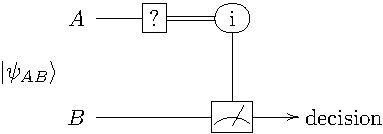
\includegraphics[width=0.9\linewidth]{gates1.pdf} 
	
	\caption{ A schematic representation of the setup for distinguishing
		measurements using entangled states. One of two known measurements $\mathcal{S}$
		or $\TT$ is performed on part $A$ of the input state $\ket{\psi_{AB}}$. We use
		the output label $i$ and perform a conditional binary measurement
		$\mathcal{R}_i$ on part $B$. By the use of its output we formulate our guess, 
		that is we decide  
		weather
		the measurement performed on part $A$ was $\mathcal{S}$ or $\TT$.
	}\label{fig:diamond}
\end{figure}



\newpage
\section{Problem formulation } 
Consider two von Neumann measurements $\PP_U$ and $\PP_{\Id}$ for  \begin{equation}
U = H_2 \left(\begin{array}{cc}1&0\\0&e^{i \phi}\end{array}\right)  H_2^\dagger,
\end{equation}
where
$U$ is unitary matrix parameterized by angle $\phi \in [0, 2\pi)$ and $H_2$ is Hadamard matrix. 

\subsection{Holevo-Helstrom theorem}
The celebrated result by Helstrom gives an upper
bound on the probability of correct distinction between two von Neumann measurements
$\PP_U$ and $\PP_{\Id}$ in terms of their distance with the use of the diamond norm
\begin{equation}
p \leq \frac12 + \frac14 \| \PP_U - \PP_{\Id} \|_\diamond.
\end{equation}





\begin{theorem}(Tw. 1 from \cite{puchala2018strategies})\label{th:minE}
	Let $U\in \UU_d$ and let $\PP_U$ and $\PP_\Id$ be two von Neumann 
	measurements. 
	Let also 
	$\diaguni_d$ be the set of diagonal unitary matrices of dimension $d$. Then
	\begin{equation}
	\|\PP_U - \PP_\Id\|_\diamond = \min_{E \in \diaguni_d} \|\Phi_{UE} - 
	\Phi_\Id\|_\diamond,
	\end{equation}
	where $\Phi_U$ is unitary channel.
\end{theorem}


\subsection{Discrimination of unitary channels}

Before we proceed to presenting our main results, we need to briefly discuss the
problem of discrimination of unitary channels. This can be done without the
usage of entangled input. In order to formulate the condition for perfect
discrimination of unitary channels we introduce the notion of numerical range of
a matrix $A \in M_d$, denoted by $W(A) =\{\bra{x}A\ket{x}: \ket{x} \in \C^d, \;
\;\braket{x}{x}=1\}$. The celebrated Hausdorf-T\"oplitz
theorem states that
$W(A)$ is a convex set and therefore $W(A) =\{\tr A \sigma : \sigma \in \Omega_d
\}$. Let us now recall the well-known result for the
distinguishability of unitary channels.
	Let $U \in \UU_d$ and $\Phi_U: \rho \mapsto U \rho U^\dagger$ be a unitary 
	channel. 
	Then 
	\begin{equation}
	\| \Phi_U  - \Phi_{\1} \|_\diamond = 2 \sqrt{1-\nu^2},
	\end{equation}
	where $\nu = \min_{x \in W(U^\dagger)} |x|  $. 

\begin{proposition}
 Let $U = H_2 \diag(1, e^{i \phi}) H_2^\dagger$, $\phi \in [0, 2\pi)$ and	let 
 $\Phi_U$ and $\Phi_\Id$ be two unitary channels. The following equation holds 
	\begin{equation}
	\min_{E \in \diaguni_2} \|\Phi_{UE} - 
	\Phi_\Id\|_\diamond = \|\Phi_{U} - 
	\Phi_\Id\|_\diamond
	\end{equation}
\end{proposition}
\begin{proof} We know that
$
	\| \Phi_U  - \Phi_{\1} \|_\diamond = 2 \sqrt{1-\nu^2},
$
	where $\nu = \min_{x \in W(U^\dagger)} |x|  $. For $U = H_2 \left(\begin{array}{cc}1&0\\0&e^{i \phi}\end{array}\right)  H_2^\dagger$ we obtain that $\nu = \frac{|1 + e^{i \phi} | }{2}$. 
	The condition $ 	\min_{E \in \diaguni_2} \|\Phi_{UE} - 
	\Phi_\Id\|_\diamond = \|\Phi_{U} - 
	\Phi_\Id\|_\diamond $ is equivalent to prove that
	\begin{equation}
	\max_{E \in \diaguni_2 } \nu_E = \nu = \frac{|1 + e^{i \phi} | }{2},
	\end{equation}
	where $\nu_E = \min_{x \in W(U^\dagger E)} |x|. $ We can prove that
	\begin{equation}
	\min_{\ket{x} \in \CC^2  \proj{x} = 1} |\bra{x}U^\dagger\ket{x}| = \min_{\rho \in \Omega_2} |\tr(U^\dagger\rho)|. 
	\end{equation}
For that, to calculate $\nu_E$ we obtain \begin{equation}
	\max_{E \in \diaguni_2 } \nu_E  = \max_{E \in \diaguni_2 }  \min_{\rho \in \Omega_2} \left| \tr \rho U E  \right|
\end{equation}
For that, our task is reduce to show that
	\begin{equation}
	\forall E \in \diaguni_2 \,\, | \tr \rho U E | \le \nu. 
	\end{equation}
	Let us define $E = \left(\begin{array}{cc}E_0&0\\0&E_1\end{array}\right)  $ and let us take $\rho = \left(\begin{array}{cc}\frac{1}{2}&0\\0&\frac{1}{2}\end{array}\right) $. 
	From spectral theorem, let us note $U$ as
	\begin{equation}
	U= \lambda_1 \ketbra{x_1}{x_1} + \lambda_2 \ketbra{x_1}{x_2}, 
	\end{equation}
	where  for eigenvector $\lambda_1 = e^{\mathbf{i} \phi}$ the eigenvector is of the form $\ket{x_1} = \left[\begin{array}{c}\frac{1}{\sqrt{2}}\\-\frac{1}{\sqrt{2}}\end{array}\right]$, whereas for  $\lambda_2 = 1$ we have $\ket{x_2} = \left[\begin{array}{c}\frac{1}{\sqrt{2}}\\\frac{1}{\sqrt{2}}\end{array}\right]$.
	
	Then we have 
	\begin{equation}
	\begin{split}
	& \forall E \in \diaguni_2 \,\,\, | \tr \rho U E | = \frac{1}{2}  \left| \tr H_2 \diag(1, e^{i\phi}) H_2^\dagger E \right| =  \\ &
	\frac{1}{2} \left| \tr\left((  e^{i \phi} \proj{x_1} + 1 \proj{x_2} ) E \right) \right|  = 
	\frac{1}{2} \left| e^{i \phi}  \bra{x_1} E \ket{x_1} + \bra{x_2} E \ket{x_2} \right| = \\& 
	\frac{1}{2} \left| \frac{E_0 + E_1}{2} + e^{i \phi } \frac{E_0+E_1}{2} \right| = 
	\frac{\left| 1+ e^{i \phi } \right|}{2} \left| \frac{E_0 + E_1}{2} \right| \le \nu, 
		\end{split}
	\end{equation}
	which completes the proof.
\end{proof}

\begin{remark}
	The probability of correct discrimination of von Neumann measurements 
	$\PP_U$ and $\PP_{\Id}$ for $U = H_2 \diag(1, e^{i \phi}) H_2^\dagger$, 
	where $\phi \in [0, 2\pi)$ is given by
	\begin{equation}
	p \le \frac{1}{2} + \frac{|1 - e^{i \phi}  |}{4} . 
	\end{equation}
\end{remark}

\subsection{Form of discriminator}
On the other hand, for Hermiticity-preserving $\Phi$, we have the following 
alternative formula for the diamond norm

\begin{equation}\label{eqn:diamond-sqrt}
\|  \Phi \|_\diamond = \max_\rho \left\|(\1\otimes \sqrt{\rho}) J(\Phi) 
(\1\otimes 
\sqrt{\rho})\right\|_1.
\end{equation}
The state $\rho$, for which $\|  \Phi \|_\diamond=\left\|(\1\otimes 
\sqrt{\rho}) 
J(\Phi) (\1\otimes 
\sqrt{\rho})\right\|_1$, will be called a \textit{discriminator}.




\begin{theorem}\label{rozrpomiarow}
Let us $\mathcal{P}_U, \mathcal{P}_\1$ be two von Neumann measurements,  $U = H_2 \diag(1, e^{i \phi}) H_2^\dagger$, $\phi \in [0, 2\pi)$ such that $0 \not\in W(U)$.  If there exists the discriminator $\rho \in \Omega_2$ of the form $\rho = \frac{1}{2}\rho_1 + \frac{1}{2} \rho_2$ such that
	\begin{enumerate}
		\item $\rho_1,\rho_2 \in \Omega_2$
		\item $\Pi_1 \rho_1 \Pi_1 = \rho_1$,
		\item $\Pi_2 \rho_2 \Pi_2 = \rho_2$,
		\item  $\mathrm{diag}(\rho_1) = \mathrm{diag}(\rho_2)$,
	\end{enumerate}
	where $\Pi_1,\Pi_2 $ are the projectors on the subspaces
	spanned by the eigenvectors corresponding to $\lambda_1$ and $\lambda_2$ of $U$. Then  we have 
	\begin{equation}
	||\mathcal{P}_U - \mathcal{P}_\Id||_\diamond = 2\sqrt{1- \left|\frac{1+e^{i \phi}}{2}\right|^2}.
	\end{equation}
	%gdzie $\lambda_1, \lambda_n$ jest odpowiednio najmniejszą i największą wartością własną $U\in \mathrm{U}(\XX)$.
\end{theorem}
\begin{proof} From \ref{th:minE} we have 
	\begin{equation}
	\begin{split}
	||\mathcal{P}_U - \mathcal{P}_{\1}||_\diamond =\min_{E \in \diaguni_2} ||\mathcal{P}_{UE} - \mathcal{P}_{\1}||_\diamond = \min_{E \in \diaguni_2}|| \Delta \left(\Phi_{E^\dagger U^\dagger} - \Phi_{\1} \right) ||_\diamond \le \\ \le \min_{E \in \diaguni_2} ||\Delta||_\diamond || \Phi_{E^\dagger U^\dagger} - \Phi_{\1}  ||_\diamond \le \min_{\diaguni_2}|| \Phi_{E^\dagger U^\dagger} - \Phi_{\1} ||_\diamond.
	\end{split}
	\end{equation}
The diamond norm between two unitary channels can be calculated by 
	\begin{equation}
	\min_{E \in \diaguni_2}||\Phi_{E^\dagger U^\dagger} - \Phi_\1||_\diamond  = \min_{E \in \diaguni_2} 2\sqrt{1 - \min_{\rho \in \Omega_2} |\tr(UE \rho )|^2}.
	\end{equation}
Hence,  it is enough to calculate the formula
\begin{equation}
\begin{split}
\min_{E \in \diaguni_2} 2\sqrt{1 - \min_{\rho \in \Omega_2} |\tr(UE \rho )|^2}.
\end{split}
\end{equation}
Recall, let us note $U$ as
\begin{equation}
U= \lambda_1 \ketbra{x_1}{x_1} + \lambda_2 \ketbra{x_1}{x_2}, 
\end{equation}
where  for eigenvector $\lambda_1 = e^{\mathbf{i} \phi}$ the eigenvector is of the form $\ket{x_1} = \left[\begin{array}{c}\frac{1}{\sqrt{2}}\\-\frac{1}{\sqrt{2}}\end{array}\right]$, whereas for  $\lambda_2 = 1$ we have $\ket{x_2} = \left[\begin{array}{c}\frac{1}{\sqrt{2}}\\\frac{1}{\sqrt{2}}\end{array}\right]$. 
Consider two cases:

	$1^\circ$ Consider $\phi = \pi$. Then $U$ is of the form
	\begin{equation}
	U = \left(\begin{array}{cc}0&1\\1&0\end{array}\right).
	\end{equation}
Then $0 \in W(U)$. 	From Proposition 3 in ~\cite{puchala2018strategies} the measurements $\mathcal{P}_U, \mathcal{P}_\1$ are perfectly distinguishable if and only if there exists $\rho \in \Omega_2$ such that
	\begin{equation}
	\mathrm{diag}\left(U^\dagger \rho\right) = 0.
	\end{equation}
Hence, for $U $ we have 
	\begin{equation}
	0 = \mathrm{diag}\left(U^\dagger \rho\right) = \mathrm{diag} \left(\left(\begin{array}{cc}0&1\\1&0\end{array}\right)\left(\begin{array}{cc}\rho_{1,1}&\rho_{1,2}\\\rho_{2,1}&\rho_{2,2}\end{array}\right)\right) =  \mathrm{diag} \left(\begin{array}{cc}\rho_{2,1}&\rho_{2,2}\\\rho_{1,1}&\rho_{1,2}\end{array}\right).
	\end{equation}
 It implies that $\rho_{2,1}=\rho_{1,2} = 0$. Therefore $\rho \in \Omega_2$ for which $\mathcal{P}_U, \mathcal{P}_\1$  are perfectly distinguishable is of the form
	\begin{equation}
	\rho = \left(\begin{array}{cc}\rho_{1,1}&0\\0&\rho_{2,2}\end{array}\right),
	\end{equation}
	where $\rho_{1,1},\rho_{2,2} \ge 0$ and  $\rho_{1,1}+\rho_{2,2}=1$.

	$2^\circ$ Consider  $\phi \not = \pi$. 
The spectrum of $U$ is of the form $\sigma(U) = \{e^{\mathbf{i} \phi},1\}$. Hence $0 \not\in W\left(U\right)$.  Let us note $U$ as 
	\begin{equation}
	U= \lambda_1 \ketbra{x_1}{x_1} + \lambda_2 \ketbra{x_1}{x_2}.
	\end{equation}
Based on Lemma 5 in~\cite{puchala2018strategies} let us take $\rho_1 = \ketbra{x_1}{x_1}$ and $\rho_2 = \ketbra{x_2}{x_2}$. Obviously,  $\rho_1,\rho_2 \in \Omega_2$ and satisfies the requirements of theorem. Hence, the discriminator $\rho \in \Omega_2$ has the form 
	\begin{equation}
	\rho = \frac{1}{2} \rho_1 + \frac{1}{2}\rho_2 = \left(\begin{array}{cc}\frac{1}{2}&0\\0&\frac{1}{2}\end{array}\right)
	\end{equation}
%and 
%	\begin{equation}
%	||\mathcal{P}_U - \mathcal{P}_{\1}||_\diamond = 2 \sqrt{1 - \left| \frac{1 + e^{\mathbf{i} \phi}}{2}\right|^2 },
%	\end{equation}

	
%	
%	$1^\circ$ For $E = \1_\XX$ and $\rho  = \frac{1}{2} \rho_1 + \frac{1}{2} \rho_2$ we have 
%	\begin{equation}
%	\tr \left(U\rho \right) = \frac{1}{2} \lambda_1 \tr\left(\rho_1 \Pi_1 \right) + \frac{1}{2} \lambda_2 \tr\left(\rho_2\Pi_2 \right) = \frac{\lambda_1+\lambda_2}{2}. 
%	\end{equation}
%	Therefore, we have
%	\begin{equation}
%	2\sqrt{1 -  |\tr(UE \rho )|^2} =  2 \sqrt{1- \left|\frac{\lambda_1+\lambda_2}{2}\right|^2}.
%	\end{equation}
%	$2^\circ$ Let us consider  $E \in \diaguni_2$ given by $E = \sum_{i=1}^2 e_i \ketbra{i}{i}$   and $\rho  = \frac{1}{2} \rho_1 + \frac{1}{2} \rho_2$. Then we have 
%	\begin{equation}
%	\begin{split}
%	\tr \left(UE\rho \right) &= \frac{1}{2}\lambda_1 \tr \left(\rho_1 \Pi_1 E \right) + \frac{1}{2}\lambda_2 \tr \left(\rho_2 \Pi_2 E \right) = \\& = \frac{1}{2} \lambda_1 \sum_{i =1}^2 \bra{i}\rho_1 \ket{i} e_i + \frac{1}{2} \lambda_2 \sum_{i =1}^2 \bra{i}\rho_2 \ket{i} e_i = \frac{1}{2} \left(\lambda_1 + \lambda_2\right)\sum_{i=1}^2 \bra{i}\rho_1 \ket{i} e_i.
%	\end{split}
%	\end{equation} 
%So we have 
%	\begin{equation}
%	\left|\tr\left(UE \rho \right) \right| = \left|\frac{\lambda_1+\lambda_2}{2} \right| \cdot \left| \sum_{i=1}^2 \bra{i}\rho_2 \ket{i} e_i \right| \le \left|\frac{\lambda_1+\lambda_2}{2} \right|.
%	\end{equation}
%	It implies that
%	\begin{equation}
%	\sqrt{1 - \left|\frac{\lambda_1+\lambda_2}{2}\right|^2} \le \sqrt{1 -  |\tr(UE \rho)|^2} \le\sqrt{1 - \min_{\rho \in\Omega_2} |\tr(UE \rho )|^2}.
%	\end{equation}
%	Hence we obtain
%	\begin{equation}
%	\begin{split}
%	||\mathcal{P}_U - \mathcal{P}_{\1}||_\diamond &=  \max_{\rho \in \Omega_2} \sum_{i=1}^2  \sqrt{\left(\bra{u_i}\rho\ket{u_i} + \bra{i} \rho \ket{i} \right)^2 - 4|\bra{i}\rho\ket{u_i}|^2} \le \\& \le 2 \sqrt{1 -\left|\frac{\lambda_1+\lambda_2}{2} \right|^2}
%	\end{split}
%	\end{equation}
For $\rho =  \frac{1}{2} \rho_1 + \frac{1}{2} \rho_2$ we obtain
	\begin{equation}
	\begin{split}
	||\mathcal{P}_U - \mathcal{P}_{\1}||_\diamond &= \sum_{i=1}^2  \sqrt{\left(\bra{u_i}\rho\ket{u_i} + \bra{i} \rho \ket{i} \right)^2 - 4|\bra{i}\rho\ket{u_i}|^2} = \\& \sum_{i=1}^2  \sqrt{\left(\bra{i}U^\dagger\rho U \ket{i} + \bra{i} \rho \ket{i} \right)^2 - 4|\bra{i}\rho U \ket{i}|^2} = \\& \sum_{i=1}^2  \sqrt{4 \bra{i}\rho \ket{i}^2 - 4 \left| \frac{\lambda_1 \bra{i}\rho_1 \ket{i} + \lambda_2\bra{i} \rho_2\ket{i}}{2}\right|^2} =\\&  \sum_{i=1}^2  \sqrt{4 \bra{i}\rho \ket{i}^2 - 4 \bra{i} \rho \ket{i} \left| \frac{\lambda_1 + \lambda_2}{2}\right|^2} = \\&  \sum_{i=1}^2 2 \bra{i} \rho \ket{i} \sqrt{1 -\left| \frac{\lambda_1 + \lambda_2}{2}\right|^2 } = \\& 2 \sqrt{1 -\left| \frac{\lambda_1 + \lambda_2}{2}\right|^2 } = 
	2 \sqrt{1 -\left| \frac{1+e^{i \phi}}{2}\right|^2 } ,
	\end{split}
	\end{equation}
which completes the proof.
\end{proof}


\begin{remark}\label{lemma:rho}
	Let $\rho_{0} = \frac{1}{2} 
	\left(\begin{array}{cc}1&0\\0&1\end{array}\right)$. Then 
	\begin{equation}
	 \max_\rho \left\|(\1\otimes \sqrt{\rho}) J(\PP_U - \PP_{\Id}) 
	(\1\otimes 
	\sqrt{\rho})\right\|_1 =    \left\|(\1\otimes \sqrt{\rho_0}) J(\PP_U - 
	\PP_{\Id}) 
		(\1\otimes 
		\sqrt{\rho_0})\right\|_1
	\end{equation}
	for  $U = H_2\diag(1, e^{i \phi}) H_2^\dagger $, 
		where $\phi \in [0, 2\pi)$. 
\end{remark}

\begin{scheme}\label{remark:discriminator}

Let us consider the problem of discrimination of von Neumann measurements 
$\PP_U$
and $\PP_{\Id}$ for $U = H_2 \diag(1, e^{i \phi}) H_2^\dagger$, 
	where $\phi \in [0, 2\pi)$. The schematic representation of theoretical 
	setup is shown in Fig.~\ref{fig:theoretical}. 

From ~\cite{puchala2018strategies}(Proposition 4) and Lemma~\ref{lemma:rho} we 
have 
	\begin{equation}
	\ket{\psi} = | \sqrt{\rho}^\top \rangle \rangle = \frac{1}{\sqrt{2}} |\Id_2 
	\rangle \rangle. 
	\end{equation}
	From Holevo-Helstrom theorem  we constrain a measurement $\mu$.  
	Let us define \begin{equation}
	X  = \left( \PP_U \otimes \Id_2 \right)(\proj{\psi}) -  \left( \PP_\Id 
	\otimes \Id_2 \right)(\proj{\psi})
	\end{equation}
	where $\ket{\psi}$ is defined in Remark~\ref{remark:discriminator}. From 
	Hahn-Jordan decomposition let \begin{equation}
	X = P - Q
	\end{equation}
	where $P, Q \ge 0 $. Observe, that $P $ and $Q$ are block-diagonal. 
	Let us define projectors $\Pi_P$ and $\Pi_Q$ onto  $im(P)$ and $im(Q)$, 
	respectively. Then  $\Pi_P$ and $\Pi_Q$ have the following forms
	\begin{equation}
	\Pi_P = \left(\begin{array}{cc}\proj{x_p}&0\\0&\proj{y_p}\end{array}\right) 
	\end{equation}
	and 
	\begin{equation}
	\Pi_Q = \left(\begin{array}{cc}\proj{x_q}&0\\0&\proj{y_q}\end{array}\right) 
	\end{equation}
	Hence, we define $V_0$ such that
	\begin{equation}
	\begin{split}
	V_0 \ket{x_p} = \ket{0} \\ 
	V_0 \ket{x_q} = \ket{1}
	\end{split}
	\end{equation}
	and $V_1$ such that
	\begin{equation}
	\begin{split}
	V_1 \ket{y_p} = \ket{0} \\ 
	V_1 \ket{y_q} = \ket{1}
	\end{split}
	\end{equation}
	The explicit form of $V_0$ and $V_1$ we can see in \texttt{one-qubit.nb}.
	Finally, we obtain the measurement $\mu$ of the form
	\begin{equation}
	\begin{split}
	 \mu(0) = \proj{0} \otimes V_0 \proj{0} V_0^\dagger +  \proj{1} \otimes V_1 
	 \proj{0} V_1^\dagger  \\ 
	\mu(1) = \proj{0} \otimes V_0 \proj{1} V_0^\dagger +  \proj{1} \otimes V_1 
	\proj{1} V_1^\dagger  
	\end{split}
	\end{equation}
\end{scheme}
This scheme is only theoretical. It is not possible to implement it on Rigetti 
architecture. For this, we will consider two approaches. The first one is 
described  by using postselection whereas the second one is considered by implementation 
of controlled unitary gate. 
%%%%%%%%%%%%%%%%%%%%%%%%%%%%%%%%%%%%%%%%%%%%%%%%%%%%%%%%%%%%%%%%%%%%%%%%%%%%%%%%

\subsection{Construction of $V_0$ and $V_1$}
	For each $\phi \in \R$,  the controlled unitary $V_0$ and $V_1$ have the following form
	\begin{equation}
	V_0 = \left(\begin{array}{cc}i \sin\left( \frac{\pi - \phi}{4} \right)&-i \cos\left( \frac{\pi - \phi}{4} \right)\\ \cos\left( \frac{\pi - \phi}{4}\right)& \sin\left( \frac{\pi - \phi}{4} \right)\end{array}\right),
	\end{equation}
	
		\begin{equation}
	V_1 = \left(\begin{array}{cc}-i \cos\left(\frac{\pi - \phi}{4}\right) &i \sin\left( \frac{\pi - \phi}{4}\right)\\\sin\left( \frac{\pi - \phi}{4} \right) &  \cos\left( \frac{\pi - \phi}{4} \right) \end{array}\right).
	\end{equation}
	
\newpage
\begin{scheme}(By using postsellection)

\begin{enumerate}
\item We prepare input state $\ket{\psi} = \frac{1}{\sqrt{2} } | \Id_2 \rangle 
\rangle. $
\item We prepare one of two unitary channel $\Phi_{U} $ or $\Phi_{\1}$. 
\item We implement unitary $V_0 $ or $ V_1$.
\item We prepare the measurement $\Delta$ in standard basis (already exists on 
Rigetti architecture) on each qubits.
\item We calculate the probability of correct discrimination in the following 
way
\begin{equation}
p = ...
\end{equation}
\todo[inline]{grubsza kmina, musze Ci to na zywo opowiedziec xd}
\end{enumerate}
\end{scheme}


\newpage
\begin{scheme}(By using controlled unitary)

\begin{enumerate}
\item We prepare input state $\ket{\psi} = \frac{1}{\sqrt{2} } | \Id_2 \rangle 
\rangle. $
\item We prepare one of two unitary channel $\Phi_{U} $ or $\Phi_{\1}$. 
\item We implement controlled unitary $V_0 \oplus V_1$.
\item We prepare the measurement $\Delta$ in standard basis (already exist on 
Rigetti architecture) on each qubits.
\item We calculate the probability of correct discrimination in the following 
way
\begin{equation}
p = \frac{|j=0 \wedge \Phi_{U} | + |j=1 \wedge \Phi_{\1}|}{\text{all 
cases}}
\end{equation}
\end{enumerate}
\end{scheme}
%
%
%
%PyQBench to biblioteka języka Python oraz narzędzie wiersza polecenia służące do testowania bramkowych komputerów kwantowych na podstawie ich zdolności do rozróżniania pomiędzy dwoma pomiarami von Neumanna w różnych bazach. Narzędzie wiersza polecenia pozwala na uruchomienie benchmarków wykorzystujących rozróżnianie między pomiarem w bazie obliczeniowej a pomiarem w bazie definiowanej przez sparametryzowaną rodzinę Fouriera. Użytkownik może wybierać, czy eksperyment zostanie przeprowadzony przy pomocy postselekcji czy alternatywnej metody “sumy prostej”, oraz kontrolować różne aspekty przeprowadzanego eksperymentu, takie jak liczba próbek używanych w samplowaniu, indeksy kubitów, zakresy kąta dla sparametryzowanej rodziny Fouriera. Jeżeli użytkownik chce użyć pomiaru w innej bazie, może wykorzystać PyQBench jako bibliotekę. Ten tryb użycia wymaga większego nakładu pracy, ale pozwala na rozszerzenie parametrów eksperymentu.  Warto wspomnieć, że w przypadku backendów udostępniających informacje o kalibracji kubitów, PyQBench wspiera mitygację błędów metodą matrix-free measurement mitigation. 
% Jednym z testowanych komputerów kwantowych był IBMQ, na którym wykonywane zostały eksperymenty na podstawie benchmarku rozróżniania pomiarów von Neumanna. 
%Obecnie opracowujemy zebrane wyniki.
%Biblioteka PyQBench będzie otwartym oprogramowaniem (ang. open source). Niebawem również zostanie wysłany artykuł do publikacji w czasopiśmie.  
\section*{Acknowledgments}


This work was supported by the project ,,Near-term quantum computers Challenges, 
optimal implementations and applications'' under
Grant Number POIR.04.04.00-00-17C1/18-00, which is carried out within the 
Team-Net programme of the
Foundation for Polish Science co-financed by the European Union under the European Regional
Development Fund.



\bibliographystyle{ieeetr}
\bibliography{rigetti.bib}





\end{document}